\documentclass[12pt]{article}
\usepackage{amsmath}
\usepackage{graphicx}
\usepackage{hyperref}
\usepackage[utf8]{inputenc}
\usepackage{geometry}
\usepackage{mathtools}
\usepackage{empheq}
\usepackage{listings}
\usepackage{xcolor}
\usepackage{minted}
\usepackage{siunitx}
\definecolor{LightGray}{gray}{0.9}

\graphicspath{ {./} }
\geometry{margin=0.75in}

\title{CHEN 425 HW2}
\author{Mark Levchenko}
\date{January 2023}

\begin{document}

\begin{enumerate}
% Problem 1 %%%%%%%%%%%%%%%%%%%%%%%%%%%%%%%%%%%%%%%%%%%%%%%%%%%%%%%%%%%%
\newpage
    \item Problem 2.21
    \begin{align*}
        \mathrm{ROI} &= \frac{10 \mathrm{yr}}{\$ 40 \text{ MM}} \\
        \Aboxed{\mathrm{ROI} &= 25\%} \\
        \mathrm{FCI} &= \$ 40 \text{ MM} \cdot 0.85 = \$ 34 \text{ MM} \\
        \mathrm{PBP} &= \frac{\$ 34 \text{ MM}}{10 \mathrm{yr}} \\
        \Aboxed{\mathrm{PBP} &= 3.4 \mathrm{yr}}
    \end{align*}


% Problem 2 %%%%%%%%%%%%%%%%%%%%%%%%%%%%%%%%%%%%%%%%%%%%%%%%%%%%%%%%%%%%
\newpage
    \item Problem 2.22
    \begin{align*}
        \mathrm{income} &= (5 \text{ MMBTU/hr} \cdot \$4/\mathrm{BTU} + 14 \text{ MMBTU/hr} \cdot \$7/\mathrm{BTU}) \cdot 8000 \text{ hr/yr} \\
        \mathrm{income} &= \$0.944 \text{ MM/yr} \\
        \mathrm{Depreciation} &= \frac{\$ 4 \text{ MM}}{10 \mathrm{yr}} = \$0.4 \text{ MM/yr} \\
        \text{After tax income} &= (\$0.944 \text{ MM/yr} - \$0.4 \text{ MM/yr} - \$0.5 \text{ MM/yr}) \cdot (1 - 0.25) + \$0.4 \text{ MM/yr} \\
        \text{After tax income} &= \$0.433 \text{ MM/yr} \\
        \mathrm{PBP} &= \frac{\$4 \text{ MM}}{\$0.433 \text{ MM/yr}} \\
        \Aboxed{\mathrm{PBP} &= 9.24 \text{ yr}}
    \end{align*}


% Problem 3 %%%%%%%%%%%%%%%%%%%%%%%%%%%%%%%%%%%%%%%%%%%%%%%%%%%%%%%%%%%%
\newpage
    \item Problem 2.23
    \begin{align*}
        \intertext{For $i=0.15$}
        \mathrm{Depreciation} &= \frac{\$ 4 \text{ MM} - \$ 0.5 \text{ MM}}{10 \mathrm{yr}} = \$0.35 \text{ MM/yr} \\
        \mathrm{income} &= (\$1 \text{ MM/yr} - \$0.35 \text{ MM/yr} - \$0.2 \text{ MM/yr}) \cdot (1 - 0.3) + \$0.35 \text{ MM/yr} \\
        \mathrm{income} &= \$0.665 \text{ MM/yr} \\
        \mathrm{NPV} &= \$0.665 \text{ MM/yr} \cdot \left( \frac{(1+0.15)^{10}-1}{0.15\cdot(1+0.15)^{10}} \right) + \frac{\$0.4 \text{ MM} + \$0.5 \text{ MM}}{(1+0.15)^{10}} - \$4.4 \text{ MM} \\ 
        \Aboxed{\mathrm{NPV} &= - \$0.84 \text{ MM}} \\ 
        \intertext{For $i=0.1$}
        \intertext{Procedure is the same as above for $i=0.1$}
        \Aboxed{\mathrm{NPV} &= \$0.0331 \text{ MM}}
    \end{align*}

    The lower discount rate project has a higher NPV. It is desirable to have a higher discount rate because that will result in a higher NPV at the end of the project.


% Problem 4 %%%%%%%%%%%%%%%%%%%%%%%%%%%%%%%%%%%%%%%%%%%%%%%%%%%%%%%%%%%%
\newpage
    \item Problem 2.24
    \begin{align*}
        \mathrm{NPV} &= \$1 \text{ MM/yr} \cdot \left( \frac{(1+i)^{10}-1}{i\cdot(1+i)^{10}} \right) + \frac{\$0.4 \text{ MM}}{(1+i)^{10}} - \$3.6 \text{ MM} \\ 
        \intertext{Find $i$ where NPV = 0:}
        i &= 0.251 \\
        \Aboxed{\mathrm{ROI} &= 25.1\%} 
    \end{align*}

    The ROI of this project is sufficiently high for the company to invest in.


% Problem 5 %%%%%%%%%%%%%%%%%%%%%%%%%%%%%%%%%%%%%%%%%%%%%%%%%%%%%%%%%%%%
\newpage
    \item Problem 2.25

    Data from spreadsheet used for calculations calculations:
    
    \begin{tabular}{|c|c|c|c|c|}
        \hline
        Year & Cash flow (\$MM/yr) & Discount & Discounted cash flow (\$MM/yr) & NPV \\
        \hline
        0&	-40&	1&	-40&	-40 \\
        1&	-330&	0.8695&	-286.956&	-326.956 \\
        2&	-400&	0.7561&	-302.457&	-629.413 \\
        3&	261.5&	0.6575&	171.940&	-457.473 \\
        4&	440.25&	0.5717&	251.714&	-205.759 \\
        5&	440.25&	0.4971&	218.882&	13.122 \\
        6&	440.25&	0.4323&	190.332&	203.455 \\
        7&	482.5&	0.3759&	181.389&	384.844 \\
        8&	482.5&	0.3269&	157.730&	542.574 \\
        9&	365.5&	0.2842&	103.897&	646.472 \\
        10&	378.5&	0.2471&	93.5594&	740.032 \\
        11&	391.5&	0.2149&	84.1502&	824.182 \\
        12&	378.5&	0.1869&	70.7443&	894.926 \\
        \hline
    \end{tabular}

    NPV: \boxed{894.926}

    Discounted PBP: \boxed{4.35 \text{ yr}}

    Discounted ROI: \boxed{39.7\%}

    Spreadsheet screenshot:

    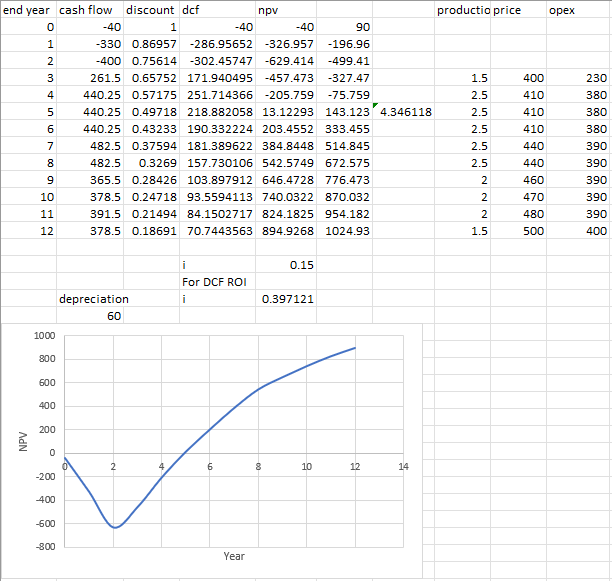
\includegraphics{2.25_spreadsheet.png}

    


% Problem 6 %%%%%%%%%%%%%%%%%%%%%%%%%%%%%%%%%%%%%%%%%%%%%%%%%%%%%%%%%%%%
\newpage
    \item Problem 2.26
    \begin{align*}
        \intertext{Base project:}
        \mathrm{ROI} &= \frac{\$1 \text{ MM/yr}}{\$5 \text{ MM}} \\
        \mathrm{ROI} &= 20\% \\
        \intertext{Base project i:}
        \mathrm{ROI} &= \frac{\$1.8 \text{ MM/yr} - \$1 \text{ MM/yr}}{\$2 \text{ MM}} \\
        \mathrm{ROI} &= 40\% \\
        \intertext{Base project i:}
        \mathrm{ROI} &= \frac{\$2.2 \text{ MM/yr} - \$1.8 \text{ MM/yr}}{\$4 \text{ MM}} \\
        \mathrm{ROI} &= 10\% \\
        \intertext{Total project i:}
        \mathrm{ROI} &= \frac{\$1.8 \text{ MM/yr}}{\$7 \text{ MM}} \\
        \mathrm{ROI} &= 25.7\% \\
        \intertext{Total project ii:}
        \mathrm{ROI} &= \frac{\$2.2 \text{ MM/yr}}{\$11 \text{ MM}} \\
        \mathrm{ROI} &= 20\% \\
    \end{align*}

    The first alternative has an ROI of 40\% which is better than the base project. This project is worth the additional investment. The second alternative has an ROI of 10\% which is less than the 20\% ROI of the base project, and thus this project is not worth the additional investment.

    The total ROI of each project is above the minimum set out by the company. However, the second project is deceptive in that its individual ROI is insufficient. If the company wants at least 15\% ROI on its investments, only the base or first project should be considered.

\end{enumerate}

\end{document}
